\documentclass[12pt]{article}

\usepackage{geometry}
\usepackage{apacite}
\usepackage{setspace}
\linespread{1.5}
\geometry{letterpaper,tmargin=1in,bmargin=1in,lmargin=1in,rmargin=1in}

\usepackage[utf8]{inputenc}
\usepackage[T1]{fontenc}
\usepackage[frenchb]{babel}

\author{a}
\title{a}
\usepackage[final]{pdfpages}
\newcommand\code[1]{\texttt{#1}}

\begin{document}
\includepdf[pages=1]{page_titre.pdf}
\setcounter{page}{1}

\tableofcontents

\section{Introduction}

\section{Présentation technique}

	Dans cette section nous présentons les diverses classes et modules impliqués
	dans l'application.  Premièrement, nous présentons quelques classes de
	librairies importantes utilisées par l'application.  Ensuite, nous
	présentons les classes que nous avons écrites pour l'application elle même.

	\subsection{Classes de librairie}

	Les classes importantes utilisées sont la classe wifiManager et ScanResult
	pour la recherche des points d'acces WiFi à proximité.  Pour la carte et
	l'API Google Maps, nous utilisons la classe GoogleMap et les classes
	GoogleMap.Marker et GoogleMap.MarkerOptions.

	\subsubsection{Classes utilisées pour le Wifi}

	La recherche de points d'accès est faite à l'aide de la classe
	\code{WifiManager}.  Celle-ci demande les points d'accès disponible au
	dispositif avec la fonction \code{getScanResults()} qui retourne une liste
	d'objet \code{ScanResult}.

	Ceci requiert une certaine mise-en-place, notament la création d'un
	\code{WifiScanReceiver} et l'enregistrement de celui-ci avec la fonction
	\code{registerReceiver()} de la classe \code{Activity}.

	\subsubsection{Classes utilisées pour les Maps}

	La classe \code{GoogleMap} est notre point d'accès aux APIs de carte
	géographique de Google.  On pose un fragment dans le \code{layout} de notre
	activté.  Ceci demande que notre classe implémente l'interface
	\code{onMapReadyCallback} qui demande que la fonction ait une méthode
	\code{onMapReady()}.


	\subsection{Classes propres à l'application}

	Dans cette section nous présentons les classes créées pour notre application
	ainsi que leurs méthodes.  Nous expliquerons aussi les choix de conception
	pertinents pour comprendre ces classes.

	Notre application fonctionne avec NN classes principales.  La plus
	importante est la classe \code{MapsActivity} qui est la classe maitresse de
	l'application.

	Parmis ses attributs, les suivants sont les plus importants:
	\begin{description}
		\item[\code{mMap}]

			Un objet de type \code{com.google.android.gms.maps.GoogleMap} qui
			nous offre la communication avec les service de Google et nous donne
			un carte géographique avec laquelle nous interagissons.

		\item[\code{PointsAcces}]

			Une liste de points d'accès trouvés par \code{WifiManager}.  La
			classe \code{PointAcces} est un adaptateur de la classe
			\code{ScanResult}.

		\item[\code{FragmentListePointsAcces}]

			Un fragment qui hérite de \code{ListFragment} et qui s'occupe
			d'afficher les éléments de notre liste de \code{PointAcces}.

		\item[\code{FragmentDetailsPointsAcces}]

			Ce fragment afficher les détails d'un \code{PointAcces} dans une
			vue et des boutons dans une autre vue.  Un fragment de ce type est
			créé lorsqu'un point d'accès est sélectionné.
	\end{description}

	Ces classes coopèrent ensemble pour changer lorsqu'un point d'accès est
	sélectionné.  La figure \ref{fig_interaction} résume les interactions qui
	arrivent lorsqu'un point d'accès est sélectionné soit en cliquant sur un
	marqueur dans la carte ou en cliquant sur un élément de la liste.

	On peut sélectionner un point d'accès en cliquant dans la liste ou en
	cliquant sur son marqueur dans la carte.  Cette action cause un appel à la
	méthode \code{onPointAccesSelected()} de \code{MapsActivity}.  Cette
	fonction remplace le fragment de droite par un fragment contenant les
	détails du point d'accès ainsi que quelques boutons pour permettre des
	actons.

	\begin{figure}[h]
		\label{fig_interaction}
		\centering
		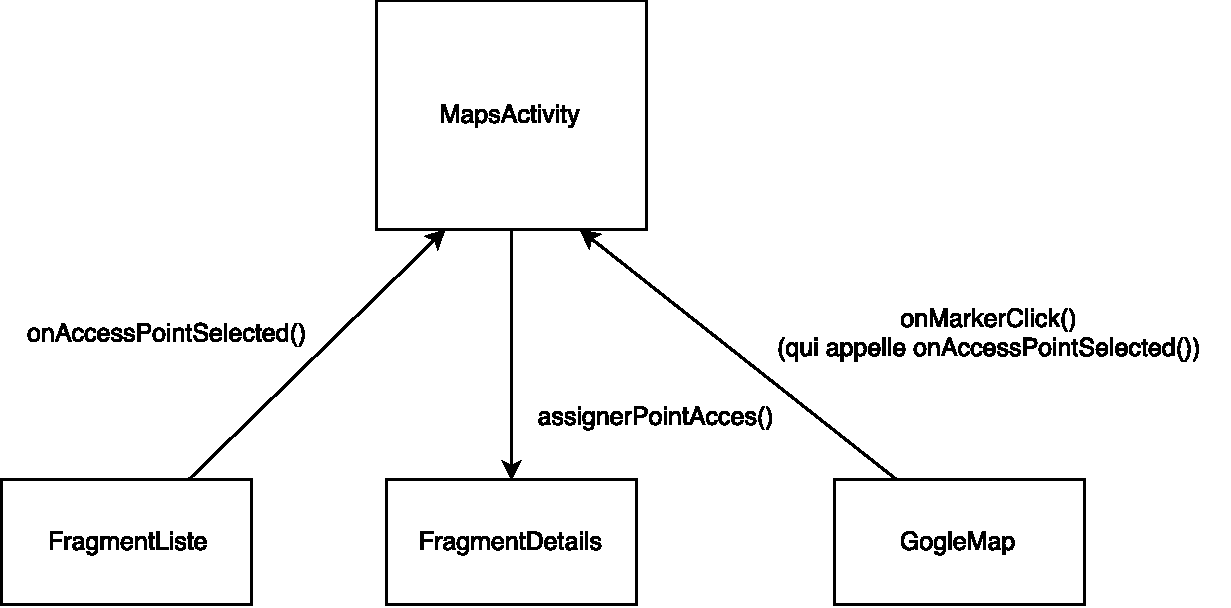
\includegraphics[height=2.5in]{communication_diag.pdf}
	\end{figure}

	% Lorsqu'un marqueur est cliqué, la fonction de rappel \code{onMarkerClick()}
	% est appelée et cette fonction appelle \code{onPointAccesSelected}.  Pour la
	% liste, elle appelle directement l




\section{Difficultés rencontrées}

	Les trois auteurs n'avaient pas d'expérience préalable avec le dévelopement
	Android.  Nous avons donc eu une bonne mesure de difficultés.  Cette section
	les énumère en détail.



\section{Critiques et suggestions}
\section{Conclusion}
Example citation: \citeA{google}.

\bibliographystyle{apacite}
\bibliography{bibdb}
\end{document}
